\documentclass[10pt]{article}

\usepackage{amsfonts}
\usepackage{amsmath,amssymb,amsthm,amsthm}
%\usepackage{mathtools}
\usepackage{dsfont}
\usepackage{etoolbox}
\usepackage[english]{babel}
\usepackage{microtype}
\usepackage{hyperref}
\usepackage{epstopdf}
\usepackage{bmpsize}
\usepackage{epsfig}
\usepackage{cleveref}
\usepackage{geometry}
\usepackage{mathrsfs}
\usepackage[affil-it]{authblk}
%\usepackage{showkeys}
\usepackage{bm}
\usepackage{pifont}
\usepackage{fleqn}
\usepackage{graphicx}
\usepackage{txfonts}
\usepackage{paralist}
\usepackage{graphics} 
\usepackage{fullpage}
\usepackage[shortcuts]{extdash}
\usepackage[leftcaption]{sidecap}
\sidecaptionvpos{figure}{m}

\usepackage{xcolor}
\usepackage{tikz}
\usepackage{pgfplots}
\usepackage{pgfplotstable}
\usepackage{subfig}
\usetikzlibrary{matrix,pgfplots.external,fit,math}
\tikzexternalize[prefix=figures/]
%\tikzset{external/force remake}

\hfuzz=4pt

\DisableLigatures{encoding = *, family = * }

\newtheorem{theorem}{Theorem}[section]

\newcommand{\norm}[2]{{\left\|#1\right\|}_{#2}}
\newcommand{\ccs}{c_{1,s}}
\newcommand{\ffl}[2]{(-d_x^{\,2})^{#1}#2}
\newcommand{\kernel}[1]{|x-y|^{#1}}
\newcommand{\ue}[1]{#1^{\,\varepsilon}}
\newcommand{\NN}{\mathbb{N}}
\newcommand{\ZZ}{\mathbb{Z}}
\newcommand{\RR}{\mathbb{R}}
\newcommand{\CC}{\mathbb{C}}
\newcommand{\TT}{\mathbf{T}}
\newcommand{\PP}{\mathcal{P}}
\newcommand{\uin}{u_{\textrm{\small in}}}
\newcommand{\Ggh}{\mathcal{G}^h_g}

\newtheorem{remark}{Remark}
\newtheorem{corollary}{Corollary}
\newtheorem{lemma}{Lemma}
\newtheorem{proposition}{Proposition}
\newtheorem{definition}{Definition}

\makeatletter
\let\@fnsymbol\@arabic
\makeatother

%\numberwithin{equation}{section}
%\numberwithin{theorem}{section}
%\numberwithin{remark}{section}
%\numberwithin{corollary}{section}
%\numberwithin{lemma}{section}
%\numberwithin{proposition}{section}
%\numberwithin{definition}{section}

\title{{\bf WKB expansion for a fractional Schr\"odinger equation}}
%
%\author{Umberto Biccari \thanks{DeustoTech, University of Deusto, 48007 Bilbao, Basque Country, Spain.}\;\;\thanks{Facultad Ingenier\'{\i}a, Universidad de Deusto, Avda Universidades 24, 48007 Bilbao, Basque Country, Spain. Email: \texttt{umberto.biccari@deusto.es}}
%\and
%Alejandro B. Aceves \thanks{Southern Methodist University, Dedman College of Humanities and Sciences, PO Box 750235, Dallas, Texas, United States. Email: \texttt{aaceves@smu.edu}}
%}
%\date{}

\author{Umberto Biccari} 
\affil{\small DeustoTech, University of Deusto, 48007 Bilbao, Basque Country, Spain.}
\affil{Facultad Ingenier\'{\i}a, Universidad de Deusto, Avda Universidades 24, 48007 Bilbao, Basque Country, Spain. \\ Email: \texttt{umberto.biccari@deusto.es}}

\author{Alejandro B. Aceves}
\affil{\small Southern Methodist University, Dedman College of Humanities and Sciences, PO Box 750235, Dallas, Texas, U.S. \\ Email: \texttt{aaceves@smu.edu}}

\date{}

\begin{document}
	
\bibliographystyle{acm}
	
\maketitle 

In recent years, the study of fractional integro-differential equations applied to physics and other areas has faced an extensive growth. In this framework, in the early 2000 Laskin started considering extensions of the classical quantum mechanics theory, based on the idea of replacing the classical Brownian trajectories in Feynman path integrals by Levy flights, which are generated by fractional Laplacians (\cite{laskin2000quantum,laskin2000fractional,laskin2002fractional}). This gave birth to Fractional Quantum Mechanics (FQM), which is the theory of quantum mechanics based on the fractional Schr\"odinger equation (FSE), instead than on the classical integer one. 
 
Later on, these kind of models found applications in several branches of physics, such as the study of condensed-matter realizations of L\'evy cristals (\cite{stickler2013potential}), lasers implementation (\cite{longhi2015fractional}), acoustic wave equations (\cite{liu2009recovery,tanushev2008superpositions}), gravity waves (\cite{tanushev2007mountain}), geophysics (\cite{vcerveny1982computation,hill2001prestack}).

The prototypical example of a fractional Schr\"odinger equation is given by the following one-dimensional non-local partial differential equation
\begin{align}\label{main_eq}
	\PP_s u:= \left[i\partial_t + \ffl{s}{}\right]u = 0, &\;\;  (x,t)\in\RR\times(0,+\infty), 
\end{align}
in which $\ffl{s}{}$ is the fractional Laplacian, defined for all $s\in(0,1)$ and for any function $f$ sufficiently smooth as the following singular integral
\begin{align*}
\ffl{s}{f}(x):=\ccs\; P.V. \int_{\RR}\frac{f(x)-f(y)}{\kernel{1+2s}}\,dy,
\end{align*}
with $\ccs$ a normalization constant given by 
\begin{align*}%\label{ccs}
\ccs:= \left(\int_{\RR} \frac{1-\cos(z)}{|z|^{1+2s}}\,dz\right)^{-1} = \frac{s2^{2s}\Gamma\left(s+\frac 12\right)}{\sqrt{\pi}\Gamma(1-s)},
\end{align*}
where $\Gamma$ is the usual Gamma function. 

In \cite{biccari2018wkb}, we developed a study of the propagation properties of the solutions of \eqref{main_eq}, based on a WKB analysis of the equation starting from a highly oscillatory initial datum in the form
\begin{align}\label{in_dat}
	u(x,0) = \uin(x) e^{i\frac{\xi_0}{\varepsilon} x}:=u_0(x),\;\;\; \xi_0\in\RR.
\end{align}

Here, the parameter $\varepsilon$ represents the fast space and time scale introduced in the equation, as well as the typical wavelength of oscillations of the initial datum. 

Asymptotic analysis for wave-like equations through geometric optics (also known as the Wentzel-Kramers-Brillouin (WKB) method or ray-tracing, \cite{brillouin1926mecanique,kramers1926wellenmechanik,spigler1997survey,wentzel1926verallgemeinerung}) is nowadays a classical tool that has been developed in several directions. An incomplete biography on the topic includes \cite{liu2010recovery,liu2013error,liu2015sobolev}. It is by now well-known that wave-type equations, in a local framework, have solutions that are localized near curves $(t,x(t))$ in space-time, also called rays. These curves are, in the interior of the domain of definition of the equation, solutions of a Hamiltonian system of ordinary differential equations which involves the coefficients of the operator. When one of these trajectories hits the boundary of the domain it is reflected according to the classical laws of optics.

In the case of equation \eqref{main_eq}, since $\PP_s=i\partial_t+\ffl{s}{}$ is a pseudo-differential operator with principal symbol $p_s(x,t,\xi,\tau) = \tau - |\xi|^{2s}$, the Hamiltonian system is given by
\begin{align*}%\label{char_syst}
	\begin{cases}
		\dot{x}(\sigma) = \partial_\xi p_s = \pm 2s|\xi(\sigma)|^{2s-1}, & x(0)=x_0
		\\
		\dot{t}(\sigma) = \partial_\tau p_s = 1, & t(0)=0
		\\
		\dot{\xi}(\sigma) = -\partial_x p_s = 0, & \xi(0)=\xi_0
		\\
		\dot{\tau}(\sigma) = -\partial_t p_s =0, & \tau(0)=|\xi_0|^{2s}.
	\end{cases}
\end{align*}

In addition, this system can be easily solved explicitly, and we obtain the following expressions for the bicharacteristics
\begin{align*}
	\begin{cases}
		x(\sigma) = x_0 \pm 2s|\xi_0|^{2s-1}\sigma
		\\
		t(\sigma) = \sigma 
		\\
		\xi(\sigma) = \xi_0
		\\
		\tau(\sigma) = |\xi_0|^{2s}.
	\end{cases}
\end{align*}

In particular, the rays of $\PP_s$ are given by the curves $(t,x_0\pm 2s|\xi_0|^{2s-1}t)\in(0,+\infty)\times\RR$. Notice that, as one expects since the operator has constant coefficients, these rays are straight lines.

The approach that we use for building localized solutions is quite standard. In particular, we look for quasi-solutions to \eqref{main_eq} introducing the ansatz  
\begin{align}\label{ansatz}
	\ue{u}(x,t) = \varepsilon^s e^{i\left[\xi_0\varepsilon^{-1}x\,+\,|\xi_0|^{2s}\varepsilon^{-2s}t\right]}\sum_{j\geq 0}\varepsilon^{\frac{s}{2}j}a_j\left(x,\varepsilon^{\frac{3}{2}s}t\right),
\end{align}
where the normalization constant $\varepsilon^s$ is chosen asking that the function $\ue{u}$ has $H^s(\RR)$-norm of the order $\mathcal O(1)$. The identification of the $a_j$-s is then carried out imposing
\begin{align*}
\PP_s\ue{u} = O(\varepsilon^{\infty}), 
\end{align*} 
thus obtaining a series of PDEs in which it is possible to clearly separate the leading order terms, with respect to $\varepsilon$, from several remainders which will vanish as $\varepsilon\to 0$. This generates a cascade system for the functions $a_j$, which can then be determined as the solution of certain given Partial Differential Equations. In our case, the cascade system is the following one
\begin{align}\label{cascade_system}
	\begin{cases}
		i\partial_\tau a_0 + \mathcal{C}_{\frac s2} \mathcal{D}^{\frac{s}{2}} a_0 = 0  
		\\
		i\partial_\tau a_1 + \mathcal{C}_{\frac s2} \mathcal{D}^{\frac{s}{2}} a_1 + \mathcal{C}_{s} \mathcal{D}^{s} a_0 = 0  
		\\
		i\partial_\tau a_2 + \mathcal{C}_{\frac s2} \mathcal{D}^{\frac{s}{2}} a_2 + \mathcal{C}_{s} \mathcal{D}^{s} a_1 + \mathcal{C}_{\frac{3s}{2}} \mathcal{D}^{\frac{3s}{2}} a_0(\theta,\tau) = 0, & \displaystyle x\leq\theta\leq x+\frac{\varepsilon}{\xi_0}q
		\\
		i\partial_\tau a_j + \mathcal{C}_{\frac s2}\mathcal{D}^{\frac{s}{2}}a_j + \mathcal{C}_{s} \mathcal{D}^{s}a_{j-1} + 	\mathcal{C}_{\frac{3s}{2}} \mathcal{D}^{\frac{3s}{2}}a_{j-2}(\theta,\tau) + \ffl{s}{a_{j-3}}, & j\geq 3
		\\
		&\displaystyle x\leq\theta\leq x+\frac{\varepsilon}{\xi_0}q.  
	\end{cases}
\end{align}  
with $\tau:=\varepsilon^{\frac 32 s}t$ and where $\mathcal{D}^{\,\beta}$ denotes the following fractional derivative of order $\beta$
\begin{align*}
	\mathcal{D}^{\beta} f(x):= \frac{1}{\Gamma(1-\beta)}\int_{-\infty}^x \frac{f'(y)}{(x-y)^{\beta}}\,dy.
\end{align*} 

Moreover, \eqref{cascade_system} is uniquely solvable with initial conditions imposed at $\tau = 0$ and this, of course, allows to identify the expressions of the functions $a_j$. See \cite{biccari2018wkb} for more details.

To the best of our knowledge, a WKB approach has not yet been fully developed in a non-local setting, and our work represents a first step in this direction, providing a complete procedure for obtaining a WKB expansion of equation \eqref{main_eq}. 

Our study is motivated by control problems. Indeed, it is by now well-known that geometric optics constructions for wave-like equations can be used for deriving controllability properties. These properties are usually formulated by means of an observability inequality, in which the total energy of the solutions is uniformly estimated by a partial measurement (typically, the portion of energy localized in a subset of the domain or of its boundary). In this framework, the existence of localized solutions gives sharp necessary conditions for the observability property to hold. In fact, as it was remarked by Ralston in \cite{ralston1982gaussian}, in order to observe these solutions the observation set must intersect every ray. If this were not the case, one could construct a quasi solution along a ray that would not hit the observation set and which, being negligible outside an arbitrarily small neighborhood of the ray, could not be observed. This is the so-called Geometric Control Condition (GCC), which has been proved to be almost sufficient by Bardos, Lebeau and Rauch in \cite{bardos1992sharp}, and necessary by Burq and Gérard in \cite{burq1997condition}.

In the particular case under analysis, we are able to show that given a ray $(t,x(t))$ it is possible to construct quasi-solutions of the fractional Schr\"dinger equation such that the amount of their energy outside a ball of radius $\varepsilon^{\frac 14}$ centered at $x(t)$ is of the order of $\varepsilon^{\frac 14}$. In more detail, we have the following result

\begin{theorem}\label{loc_thm}
Let $\uin\in L^2(\RR)$ and let $\ue{u}$ be constructed employing the expansion \eqref{ansatz}. Then, for any $\varepsilon>0$ we have:
\begin{enumerate}
	\item The functions $\ue{u}$ are approximate solutions to \eqref{main_eq}:
	\begin{align*}
		\norm{u_0(x)-\ue{u}(x,0)}{L^2(\RR)} = \mathcal{O}(\varepsilon^{\frac{1}{2}}),
	\end{align*}
	\begin{align*}
		\norm{u(x,t)-\ue{u}(x,t)}{L^2(\RR)} = \mathcal{O}(\varepsilon^{\frac 12}).
	\end{align*}
	\item The initial energy of $\ue{u}$ remains bounded as $\varepsilon\to 0$, i.e.
	\begin{align*}
		\norm{\ue{u}(x,0)}{H^s(\RR)}^2 \approx 1.
	\end{align*}
	\item The energy of $\ue{u}$ is exponentially small off the ray $(t,x(t))$:
	\begin{align*}
		\int_{|x-x(t)|>\varepsilon^{\frac 14}} \left|\ffl{\frac s2}{\ue{u}}(x,t)\right|^2\,dx = \mathcal O(\varepsilon^{\frac 14}).
	\end{align*}	
\end{enumerate}
\end{theorem} 

In the above theorem, the meaning of the first statement is twofold: on the one hand, we have that the function $\ue{z}$ a time $t=0$ is close, in the $L^2$-norm, to any initial datum in the form \eqref{in_dat}. On the other hand, the same remains true also for any other time $t>0$, and we have that the functions $\ue{z}$ are really approximating the real solution of \eqref{main_eq} in a $L^2$-setting.
The second statement, instead, asserts that the initial energy of $\ue{z}$, i.e. the energy at $t=0$, is essentially bounded, up to some small reminder which vanishes as $\varepsilon\to 0^+$. Also in this case, as a consequence of the energy conservation property, this same fact remains true for all times $t>0$. Finally, the third statement is possibly the most important one. Indeed, according to it the amount of energy away from a given ray of size $\varepsilon^{\frac 14}$ is of the same order $\varepsilon^{\frac 14}$. In other words, the energy which is not concentrated along $x(t)$ is negligible with respect to the total amount and, for instance, it is possible to analyze the propagation of the solutions of \eqref{main_eq} simply in terms of the propagation of the rays. 

To this end, a very important quantity for analyzing the behavior of $\ue{u}$ is the so-called \textit{group velocity}, which can be easily computed as 
\begin{align*}
	v=\left|\frac xt\right| = 2s\varepsilon^{1-2s}|\xi_0|^{2s-1}.
\end{align*}
We then immediately see that, for $s=1/2$ we have $v=1$, i.e. the velocity is constant and independent of the frequency $\xi_0$. For $s\in(0,1/2)$, instead, we have that $1-2s>0$. Hence, taking $\varepsilon<1$, we easily get
\begin{align*}
v<|\xi_0|^{2s-1}.
\end{align*}
Finally, for $s\in(1/2,1)$ the situation is the opposite. We have $1-2s<0$ and, for $\varepsilon<1$, 
\begin{align*}
v>|\xi_0|^{2s-1}.
\end{align*}
In view of these behaviors, we can conclude that:
\begin{itemize}
	\item For $s> 1/2$, the group velocity increases with the frequency.
	
	\item For $s=1/2$, the group velocity remains constant.
	
	\item For $s<1/2$, the group velocity decreases with the frequency.
\end{itemize}

Therefore, the high frequency solutions are traveling faster and faster, for $s>1/2$, and slower and slower, for $s<1/2$. This behavior has then consequences from the point of view of observation properties for the solutions. In more detail,
\begin{itemize}
	\item For $s>1/2$, the velocity of propagation of the rays allow them to be observable in any finite time $T>0$.
	\item For $s=1/2$, the velocity of propagation being constant, a minimum observation time $T_0$ is needed.
	\item for $s<1/2$ the high frequency rays may not reach the control region, thus implying the failing of controllability properties. 
\end{itemize}
This, in particular, confirms the already known results presented in \cite{biccari2014internal}.

In what follows, we present some simulations which show the propagation of solutions to the fractional Schr\"odinger equation \cref{main_eq} corresponding to initial data in the form \cref{in_dat}. 

For the numerical resolution of the equation, we employed a uniform mesh in the space variable and a FE discretization of the fractional Laplacian, obtained following the methodology presented in \cite{biccari2017controllability}. Moreover, we used a Crank-Nicholson scheme in time, which is known to be stable for the Schr\"odinger equation. The initial data $u_0$ has been chosen as  
\begin{align*}
	u_0(x) = e^{-\frac \gamma2 (x-x_0)^2}e^{i\frac {\xi_0}{\varepsilon} x},
\end{align*} 
where the profile $u_{\textrm{in}}(x)$ is given by a Gaussian with standard deviation measured in terms of the parameter $\gamma$, which is related to the mesh size $h$. In particular we chose $\gamma = h^{0.9}$. Finally, for the oscillations we considered frequencies $\xi_0=\pi^2/16$ and $\xi_0=2\pi^2$.   

In Figure \ref{plot_01}, we show the plots for $\xi_0=2\pi^2$ and different values of $s\in(0,1)$. The space domain has been chosen to be the interval $(-1,1)$, while we considered a time interval of $5$ seconds. 

\begin{figure}[!h]
	\centering 
	\begin{minipage}{0.3\textwidth}
		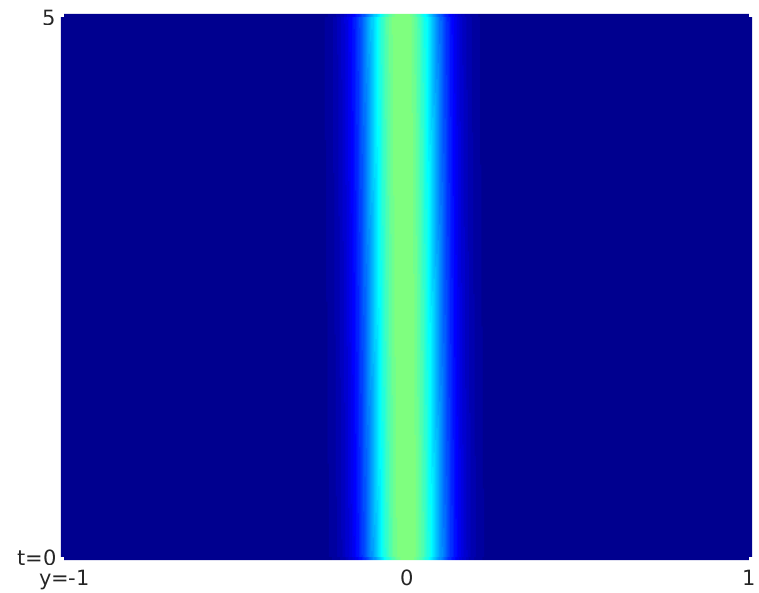
\includegraphics[scale=0.37]{./figures/plot_frac_schrodinger1_01_1}
	\end{minipage}
	\hspace{0.5cm}	
	\begin{minipage}{0.3\textwidth}
		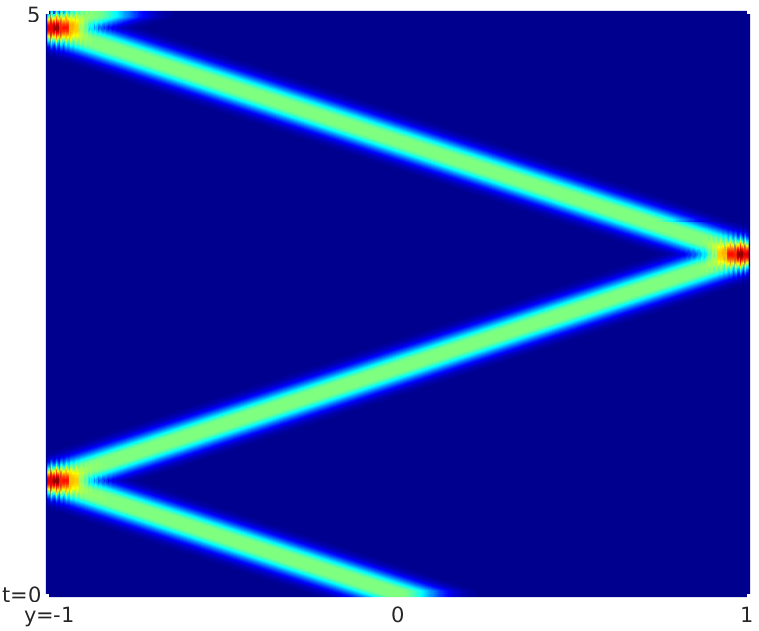
\includegraphics[scale=0.35]{./figures/plot_frac_schrodinger1_05_1}
	\end{minipage}	
	\hspace{0.2cm}	
	\begin{minipage}{0.3\textwidth}
		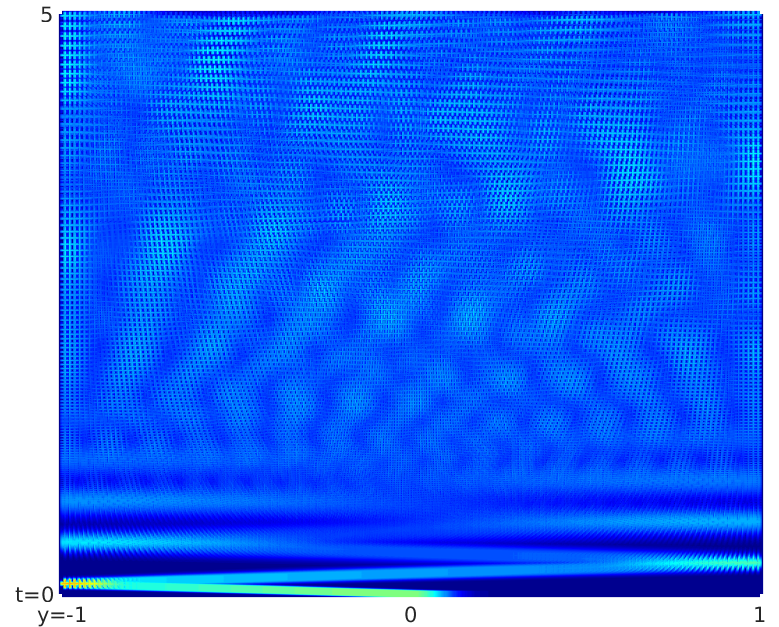
\includegraphics[scale=0.35]{./figures/plot_frac_schrodinger1_09_1}
	\end{minipage}	
	\caption{Propagation of the solution for $\xi_0 = 2\pi^2$ and different values of $s$.}\label{plot_01}
\end{figure} 

It is seen there that, for small values of $s$, say $s=0.1$, the solution remains concentrated along rays which propagate only in the vertical direction. In other words, there is no propagation in space and, as we mentioned before, this implies that it will not be possible to control these solutions, no matter how one places the controls. For $s=0.5$, instead, the plots show that the solutions propagate along rays which reach the boundary of the space domain in finite time and are reflected according to the laws of optics. This translate in the fact that, provided that the time is large enough, it will be possible to control these solutions, acting  with a control distributed in a neighborhood $\omega$ of the boundary. The case of high values of the power $s$ of the fractional Laplacian is the most puzzling one. For instance, for $s=0.9$ our plots seem to show a lost of concentration of the solution along the ray, while our theoretical results would suggest that this concentration is preserved. On the other hand, we believe that what the simulations are showing is not in contradiction with the theory. In our opinion, it is only a numerical effect, which has two possible interpretations.

First of all, for $s>1/2$, the velocity of propagation of the solutions is increasing. As a consequence, in the time framework that we are considering the waves reach the boundary and are reflected many more times than in the case $s=1/2$. This large number of reflections is quite hard to clearly distinguish a the discrete level, even when working with very fine meshes (for our simulations, for instance, we are considering a mesh of $500$ points, corresponding to a step $h$ of the order of $10^{-3}$). 
			
A second possible interpretation is that this strange phenomenon appearing in the plot can be explained with the accumulation of higher order terms in the asymptotic expansion of $\ue{z}$ which, combined with the small size of the space interval considered, enhance a chaotic behavior. This interpretation is supported by the fact that, as it is shown in Figure \ref{plot_03}, enlarging the space domain up to $(-6,6)$ it is possible to appreciate again the localization of the solution along the rays.	

In Figure \ref{plot_02}, the simulations have been run with an initial datum with frequency $\xi_0=\pi^2/16$. The plots obtained show a behavior which is totally analogous with what observed in Figure \ref{plot_01}:
\begin{itemize}
	\item For $s=0.1$, the solutions are once again concentrated along vertical rays, without propagation in time and, therefore, without possibility of being controlled.
	
	\item For $s=0.5$, we have propagation with constant velocity, and the ray reaches the boundary in finite time.
	
	\item For $s=0.9$ the chaotic comportment is still present.
\end{itemize}

\begin{figure}[!h]
	\centering 
	\begin{minipage}{0.3\textwidth}
		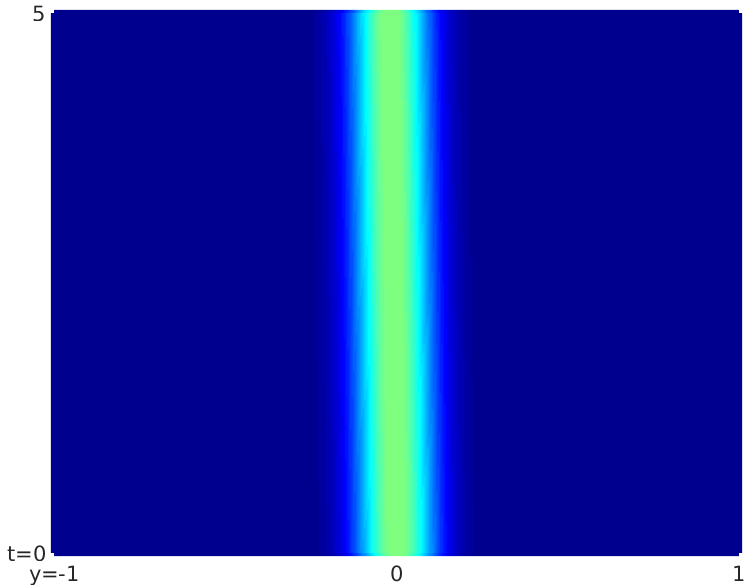
\includegraphics[scale=0.37]{./figures/plot_frac_schrodinger2_01_1}
	\end{minipage}
	\hspace{0.2cm}	
	\begin{minipage}{0.3\textwidth}
		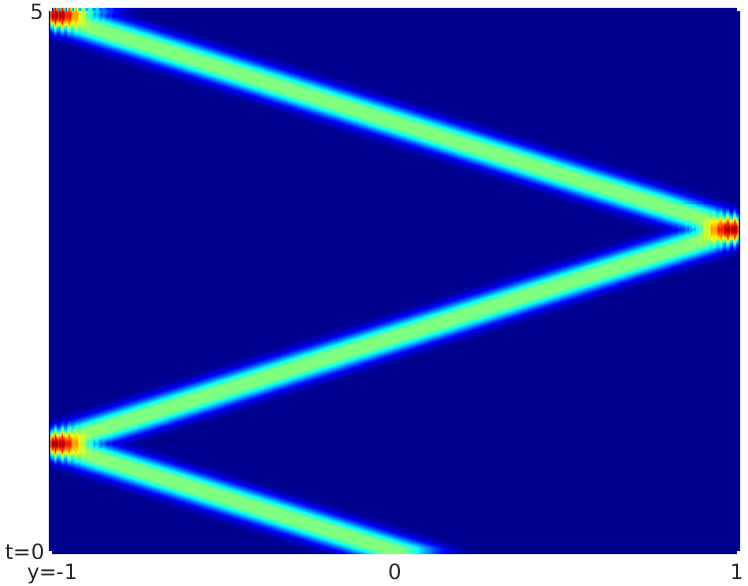
\includegraphics[scale=0.37]{./figures/plot_frac_schrodinger2_05_1}
	\end{minipage}	
	\hspace{0.2cm}	
	\begin{minipage}{0.3\textwidth}
		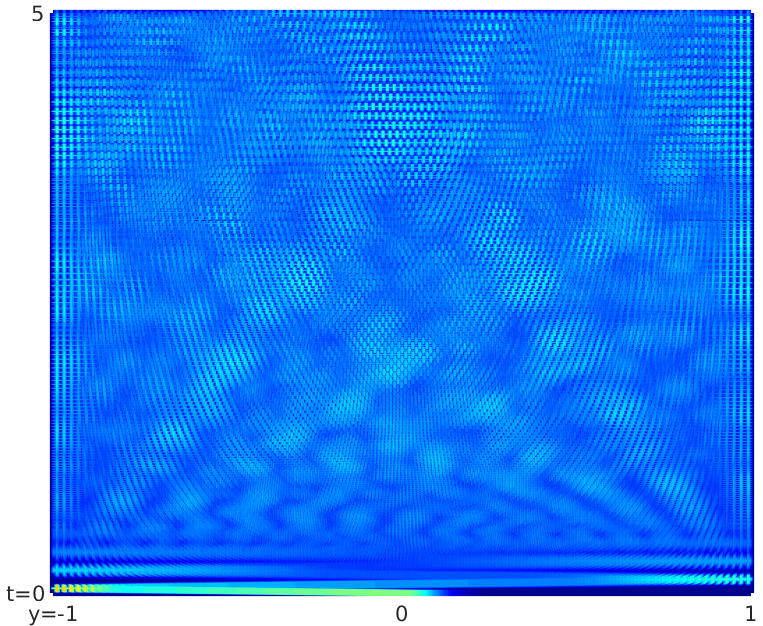
\includegraphics[scale=0.35]{./figures/plot_frac_schrodinger2_09_1}
	\end{minipage}	
	\caption{Propagation of the solution for $\xi_0 = \pi^2/16$ and different values of $s$.}\label{plot_02}
\end{figure} 

Once again, the most surprising case is the last one, for $s>0.5$, in which the simulations seem to display dispersive features. Nevertheless, as we mentioned before, we retain that this does not contradict the theoretical results, and we think that this chaotic behavior is purely a numerical effect generated by the small size of the space interval $(-1,1)$, by the high velocity of propagation of the solutions, and by the accumulation of high order terms in the asymptotic expansion. In fact, we can observe that the enlargement of the space domain up to $(-6,6)$ seems to fix the problem, and the localization of the solution along the rays appears once again (see Figure \ref{plot_03}). This, in our opinion, justifies our interpretation of the phenomenon.

\begin{figure}[!h]
	\centering 
	\begin{minipage}{0.3\textwidth}
		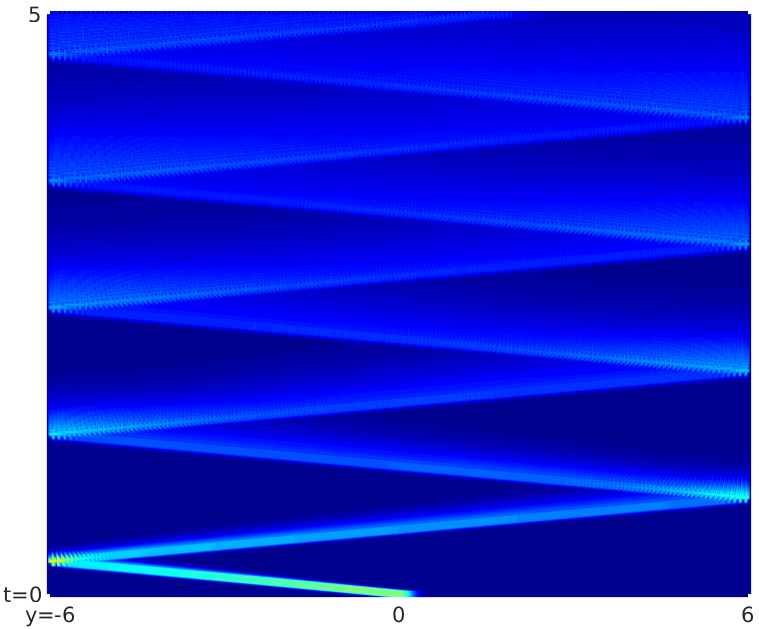
\includegraphics[scale=0.37]{./figures/plot_frac_schrodinger1_09_6}
	\end{minipage}
	\hspace{0.5cm}	
	\begin{minipage}{0.3\textwidth}
		%\vspace{0.1cm}
		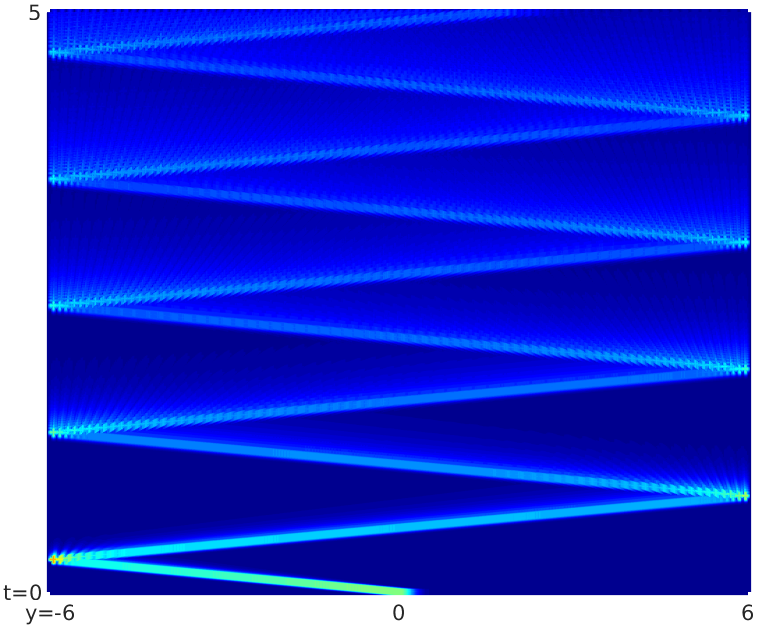
\includegraphics[scale=0.37]{./figures/plot_frac_schrodinger2_09_6}
	\end{minipage}	
	\caption{Propagation of the solution for $s=0.9$ on the space interval $(-6,6)$.}\label{plot_03}
\end{figure} 

\bibliography{biblio}
\end{document}